\begin{figure}[!h]
\centering
\resizebox{\columnwidth}{!}{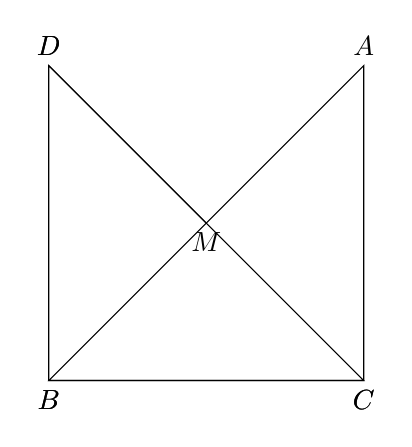
\begin{tikzpicture}
\coordinate (D) at (0,4);
\coordinate (A) at (4,4);
\coordinate (B) at (0,0);
\coordinate (C) at (4,0);
\coordinate (M) at (2,2);
\draw (A)node[above]{$A$}--(B)node[below]{$B$}--(C)node[below]{$C$}--cycle;
\draw (D)node[above]{$D$}--(B)node[below]{$B$}--(C)node[below]{$C$}--cycle;
\draw(M)node[below]{$M$}--(D)node[above]{$D$};
\tkzMarkRightAngle(D,B,C)
\tkzMarkRightAngle(A,C,B)
\end{tikzpicture}}
\caption{}
\label{eq:solutions/1/38/myfig}
\end{figure}
We are given that AB = AC. So
\begin{align}
  \norm{\vec{A-B}} = \norm{\vec{A-C}} \label{eq:solutions/1/38/eq1}
\end{align}
Also BA is produced to D such that AB = AD. Therefore we have
\begin{align}
  \vec{A-B} = \vec{D-A} \label{eq:solutions/1/38/eq2}
\end{align}
Taking dot product of vectors $\vec{(B-C)}$ and $\vec{(D-C)}$ we get
\begin{align*}
  &\vec{(B-C)}^T\vec{(D-C)}\\
  &= \vec{(B-A+A-C)}^T\vec{(D-A+A-C)}\\
  &= \vec{((B-A)+(A-C))}^T\vec{((D-A)+(A-C))}
\end{align*}
using \eqref{eq:solutions/1/38/eq2} we get
\begin{align*}
  &\vec{(B-C)}^T\vec{(D-C)} \\
  &= \vec{((B-A)+(A-C))}^T\vec{((D-A)+(A-C))}\\
  &= \vec{((B-A)+(A-C))}^T\vec{((A-B)+(A-C))}\\
  &= \vec{(-(A-B)+(A-C))}^T\vec{((A-B)+(A-C))}\\
  \begin{split}
    &= -\norm{\vec{A-B}}^2-\vec{(A-B)}^T\vec{(A-C)}\\
    &\qquad +\vec{(A-C)}^T\vec{(A-B)}+\norm{\vec{A-C}}^2
  \end{split}
\end{align*}
now $\vec{(A-B)}^T\vec{(A-C)}$ and $\vec{(A-C)}^T\vec{(A-B)}$ are both dot product of vectors $\vec{(A-B)}$ and $\vec{(A-C)}$,therefore
\begin{align*}
  &\vec{(B-C)}^T\vec{(D-C)}\\
  \begin{split}
    &= -\norm{\vec{A-B}}^2-\vec{(A-B)}^T\vec{(A-C)}\\
                                &\qquad +\vec{(A-C)}^T\vec{(A-B)}+\norm{\vec{A-C}}^2
  \end{split}\\
  &= -\norm{\vec{A-B}}^2+\norm{\vec{A-C}}^2
\end{align*}
using \eqref{eq:solutions/1/38/eq1} we get
\begin{align}
  \vec{(B-C)}^T\vec{(D-C)} &= -\norm{\vec{A-B}}^2+\norm{\vec{A-C}}^2 = 0
\end{align}
since $\vec{(B-C)}^T\vec{(D-C)}$ = 0,therefore BC $\perp$ CD and $\angle{BCD}$ is a right angle.
